\section{Problem Definition and Algorithm}

Sudoku puzzle is a relatively old classic problem. Hence, many approaches have been developed to solve Sudoku. As the focus of this project has been on AI methods, we have tried to utilize some of the classic and interesting AI methods to solve Sudoku. For instance, the solution of a Sudoku puzzle can be found using search algorithms. The more efficient the search algorithm is, the more quickly the solution is found. Sudoku is also recognized as a classic constraint satisfaction problem. The essence of Sudoku problem is based on the constraint that we have to satisfy. These constrains (see section 1). We also apply some relatively new approaches such as Convolutional Neural Network (CNN) and Genetic Algorithm to solve the Sudoku puzzles which are discussed in the following subsections respectively. 

\subsection{Uniformed Search Agent (Baseline)}
Search algorithms can be used to tackle artificial intelligence problems. Uninformed search and informed search with heuristics are two types of search algorithms. Uninformed search is a search method that is able to only differentiate between a target state and a non-goal state and has no knowledge about how distant the goal state might be from the present state []. In other words, uninformed search techniques are strategies which use a tree-traversing algorithm to search the sequence through which an agent could reach to the goal state without using any additional information. Depth-first search (DFS) and Breadth-First search (BFS) are among the uniformed search strategies. The difference is in the data structure by which they queue the nodes of the tree to visit throughout the tree-traversing process.

\subsubsection{Depth-first Search}
The Depth-fisrt search (DFS) is a popular method to be used in search problems. When a dead-end occurs in any iteration, DFS method traverses a tree in a depth-ward motion and utilizes a stack to remember to acquire the next vertex to start a search [tutorial point dfs]. We first define the terminology of a search algorithm in Sudoku context. 

\begin{itemize}
\item Node: every state of a Sudoku puzzle is represented as a node in the tree search. Each node may contain a set of cells which are already assigned a value and a set of empty cells to be filled.

\item Successor: A successor of a node inherits the current state of its parent. In addition, it has one more filled cell than its parent. That is, every state of the puzzle that its next empty cell has been filled with a valid digit which satisfies the constraints of the parent node is considered the successor of the parent node.

\item Constraint Check: To assign a value to an empty cell to create a successor, the agent must check if the new value satisfies the requirements and the constraints of the current state of the puzzle (see section 1). 

\item Goal State: The goal state is a state in which all cells of the puzzle have a valid digit and all of the constraints of the puzzle have been met.  \\

\end{itemize}

The process is started by finding the first empty cell to which we have to assign a value. We then try all values from 1 through 9 in the cell. Among all possible values, we select the values which satisfies the constraint of the Sudoku puzzle (see section 1). For each valid candidate value, we make a copy of the current state of the puzzle, assign the value to the cell and return it as a successor. It is obvious that a node can have multiple successors. We then recursively repeat the same process for all successors of the node until we reach the goal state.  Figure (1) illustrates the idea behind the DFS in Sudoku context: 

\begin{figure} [htbp]
\centering
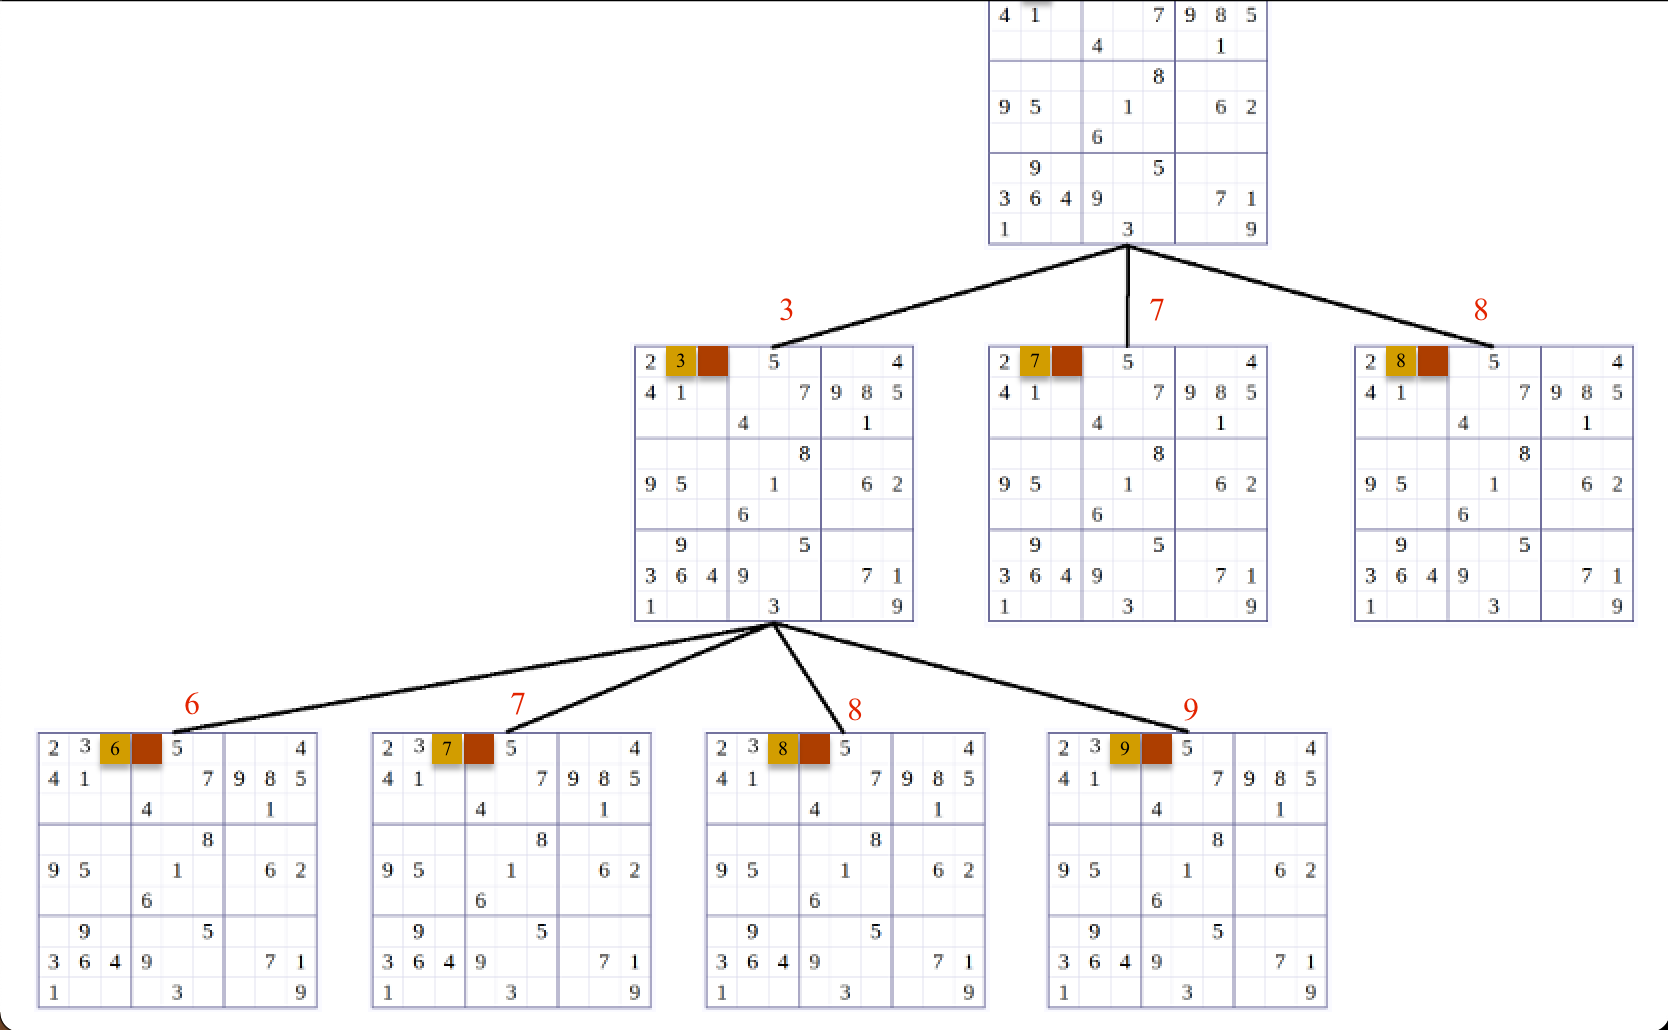
\includegraphics[width=100mm,scale=2]{figures/DFS.png}
\caption{Depth-first Search in Sudoku puzzle}
\label{fig:access_points}
\end{figure}

% \subsubsection{Breadth-first Search}
% A Breadth-First Search (BFS) is a tree-traversal technique that uses a queue rather than a stack to traverse the tree. This approach employs horizontal expansions in order to account for all possible outcomes in the Sudoku grid. The queue technique of arraying assures that all nodes are addressed, but it is also time-consuming and inefficient. In our case, this step is very similar to what we do in DFS. The only things that varies is the data structure with which we queue the nodes to be visited. As opposed to DFS whcih uses stack, BFS uses a FIFO queue for this purpose. Therefore, the order in which the new puzzles are created changes.
% In section 4, we discuss what implications the difference between DFS and BFS have on the performance of the search agent. 

\subsection{Backtracking}
Now let’s talk in more details about how we would actually approach Sudoku problem using Backtracking algorithm. Backtracking algorithms attempt to solve a problem one step at a time. If it becomes obvious at any point along the way that the present path will not lead to a solution, it will return to the previous step or backtrack and take an alternative option. 
This is known as recursive function which is used in backtracking algorithms. A recursive function is one that keeps calling itself until a certain task is completed. It tries to solve a problem by examining all potential solutions until one is identified. If a solution is not discovered each time a path is examined, the algorithm goes back to try another potential way, and so on, until a solution is found or all of the paths have been evaluated.

\subsection{Constraint Satisfaction}
To solve the sudoku puzzle, we will use PuLP package in Python.
PuLP is a python package that may be used to solve linear programming. As mentioned earlier, The essence of Sudoku puzzle is based on constraint satisfaction. It is worth mentioning that there is no optimal solution to a Sudoku problem, which means we should not look for maximization or minimization of any equations.
To solve Sudoku using constraint satisfaction techniques, we first need to define the variable of the problem. These variables depend on the nature of the constraint present in the problem. Therefore, we first look into the constraints that we have to satisfy in a Sudoku puzzle.

\textbf{Constraint 1: Each cell can only have one value} 
Only one value can be present in each cell, meaning that the other values will be absent. As a result, we may consider a binary variable with a value of 0 if the number is not there and 1 if it is. The variables looks like below:\\
\centerline{(value, row, col) = 0 or 1}\\
We should maintain the row and column variables as constant while varying the value from 1 to 9. This guarantees that every cell has just one value. Since only one parameter would be equal to 1, the rest has to be 0, the total of the binary digits should be 1.Because the row and column both have a range of 1 to 9, there are 81 permutations (row, col). There will be 9 binary variables in each combination. As a result, there are 729 variables. Only 81 of the 729 distinct pairings will have a value of 1, while the others would have a value of 0. 

\textbf{Constraint 2: Each row must have all values from 1 to 9, no repeated value}
We can maintain the value and row unchanged while changing the col from 1 to 9 in this situation.

\textbf{Constraint 3: Each column must have all values from 1 to 9, no repeated value}
Instead of maintaining value and row constant, we keep value and col constant in this constraint, which is quite similar to our prior constraint.

\textbf{Constraint 4: All values from 1 to 9 must be present in each of the 9 boxes, no repeated value.}

\textbf{Constrain 5: Set the variables for occupied cells to 1}
In Sudoku puzzles, there are usually some cells which are already assigned a value. Each value which is present at each cell is considered as a new constraint to our problem. Therefore, we set the variables (value, row, col) of already occupied cells to 1.

Finally, we solve the problem Pulp.solve() using method which solves a linear program with the defined variables and returns the solution. The linear equation created in this process is written into a file called Sudoku.lp.

\subsection{Convolution Neural Network (CNN)}

An artificial neural network is used for modelling. It is comprised of node layers, consisting of input layer, one or more hidden layer and output layer, which delivers the final output. Each node connecting to one another has a weight and threshold associated with it. If output of any individual node is above threshold, data is sent to the next layer else no data is passed along within the network. This help us to learn which notable features are there in the data to produce the output. Each of this node has its own linear regression model, consisting of data, threshold, weight, and an output.  

Convolutional neural networks, also called ConvNets are used to recognize a pattern present in images. It is a class of deep learning, feed-forward artificial neural network technique which uses a variation of multilayer perceptions designed because of which it will require minimal preprocessing. It is remarkably similar to ordinary neural network; they are made of neurons that have learnable weights and biases. Unlike NN, layers in ConvNet have neurons arranged in 3 dimensions: \textbf{height, width, and depth}. Neurons in a layer is only connected to the small region of the previous layer, instead of all the neurons in a fully connected manner. At the end of the ConvNet architecture, the full image is reduced to a single vector of class scores arranged along with the depth. A simple ConvNet is a sequence of layers, and there are three types of layers in a CNN: convolutional layer, pooling layer, and fully connected layer. 

The convolution layer is the first layer of the convolution network which can be followed by more convolution layers or pooling layers, the fully connected layer is the final layer.   

\begin{figure} [http]
\centering
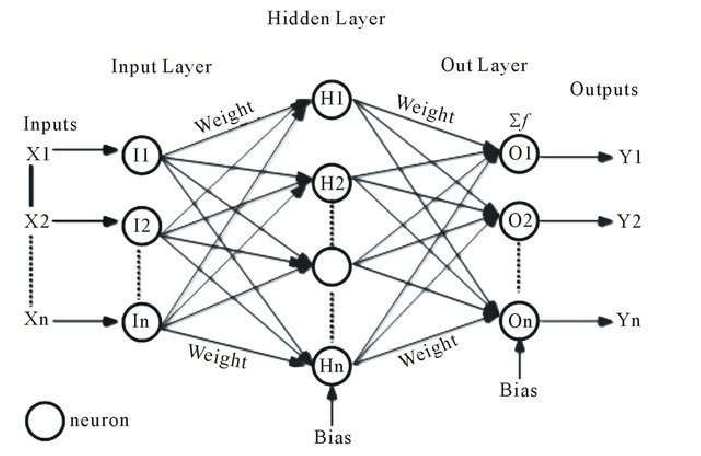
\includegraphics[width=80mm,scale=0.9]{figures/Multilayer-Perceptron-Network.png}
\caption{A schematic of an artificial neural network}
\label{fig:access_points}
\end{figure}

\subsubsection{Convolution Layer}

Convolution layer is the core of the CNN which does most of the computational heavy lifting. it requires a few components, which are input data, a filter, and a feature map. Convolution layer applies a convolution operation to the input, passing the result to the next layer, which is a linear operation which involves the multiplication between an array of input data and two-dimensional matrix of weights called a kernel (kernel is smaller than input data and the dot product is used for performing multiplication between them). The final output from the series of this dot products from the input and filter is known as activation map/feature map or convolved feature. CNN applies a Rectified Linear Unit (ReLU) transformation to the feature map after each convolution operation for introducing nonlinearity to the model. Two hyperparameters were used to control the size of the output volume – depth and zero-padding.  

\begin{itemize}
    \item Depth corresponds to the number of filters that we would like to use which will affect the depth of the output. 
    \item Zero-padding allow us to control the spatial size of the input volume, so that the shape of the input and output volume are the same. There are three types padding – Valid, Same and Full. In our case, we are using Same padding. 
\end{itemize}

\subsubsection{CallBacks}
Callback functions are defined to perform actions at various stages of training, in our case the training is stopped if there is drop in accuracy. 


\subsection{Genetic Algorithm}

\subsubsection{Generate Initial Populations:}
In the population, there is a batch of generations, which have a number of chromosomes.
The generating processing begins with generating chromosomes for each generation, each chromosome is the possible solution for Sudoku, generating the chromosome base on the given puzzle of Sudoku, chromosomes are every available element that can take place on the zero elements on a given puzzle. Evaluate initial populations by using the fitness score to assess each chromosome’s performance. Based on the Sudoku roles, every column and row should only have nine unique numbers from 1 to 9, and each 3X3 block of Sudoku should follow the same pattern. Recording every unique number as 1 in every column and blocks, if one of the numbers is duplicated, then plus record to 2. The more duplicated number, the more weight it contains in the records. the fitness score is the average duplicated column rate times duplicate block rate.

\subsubsection{Selecting Elite Generations:}
Choose the number of generations, which have better fitness scores. They include more valuable chromosomes or solutions to create new children by using the crossover. Maintain a certain amount of generations from the last population, and generate the rest of the generations as the next population. 

\subsubsection{Parents' Selection for Crossover:}
Selecting the best fittest chromosome (solution) as parent generation to crossover and pass their genes to the child generation in order to get a better solution. Two chromosomes are chosen based on their fitness scores, selecting the parent with a higher score or a low score equally, which means it has a 50 per cent of peaking the one with the higher fitness score and 50 per cent of choosing the one with a lower fitness score.

\subsubsection{Crossover:} 
Crossover is the most important step to generating get optimized generation. There are many swapping algorithms for crossover functions, such as single value crossover, row crossover, column crossover, and block crossover. In our program, we used the row crossover method on parents' chromosomes,  Swapping each element in every row in chromosomes, choosing two random rows as swapping objects to exchange their elements.

\subsubsection{Mutation:}
The mutation is another operation that optimizes the elements in chromosomes and maintains the diversity of chromosomes by checking three criteria on chromosomes that have already crossover. There are no duplicated elements in the column, no duplicated elements in the row, and no duplicated elements in the block. If two elements satisfy these criteria, then swap two elements and add children to new generations.

\subsubsection{Evaluate New Generations and Repeat:}
Check the best fittest chromosomes in generations, if the new generations have too many repeated chromosomes, it will reduce the diversity of the chromosomes, then regenerate chromosomes to avoid that. And then repeat the process from selecting elites generations until it gets the final solution, which is the fittest chromosome.
